\documentclass[11pt,show 
notes,notheorems,noamsthm,blank]{beamer} % default is 11pt
\usetheme{metropolis}
% \usepackage{beamerthemeshadow}
% \usepackage{times}
\usepackage[utf8]{inputenc}
\usepackage[scaled]{helvet} % ss
\usepackage[T1]{fontenc}
\usepackage{eurosym}
\usepackage{graphics, graphicx}
\usepackage{url}
% \usepackage{multirow}
\usepackage{listings}
\usepackage{epsfig}
%  \usepackage[portuguese]{babel}
%  \usepackage[latin1]{inputenc}  
\usepackage{fancyvrb}
\usepackage[prefix=tikzsym]{tikzsymbols}

\usepackage{fontawesome}
% \usepackage{xcolor}


% \usepackage[marvosym]{tikzsymbols}
% \usepackage{rotating}
% \usepackage{subfigure}
% \usepackage{default}
 \usepackage{algorithmic}
 \usepackage{algorithm}
\usepackage{rotating}
\usepackage{hyperref}
\definecolor{links}{HTML}{FF5050}
\definecolor{inlinks}{HTML}{4D94FF}
\hypersetup{colorlinks,linkcolor=inlinks,urlcolor=links}
\beamertemplatetransparentcovered
%  \usepackage[portuguese]{babel}
%  \usepackage[latin1]{inputenc}  
\usepackage{rotating}
\usepackage{colortbl}
% \usepackage{moreverb}
% \usepackage{tikz}
% \usepackage{wrapfig}
\setbeamertemplate{bibliography item}{\insertbiblabel}
% \usepackage{tikz}
% \usetikzlibrary{arrows,positioning,shapes}
% \usetikzlibrary{shapes,calc,shadows}
\pgfdeclarelayer{background}
\pgfdeclarelayer{foreground}
% \pagestyle{fancy}
\pgfsetlayers{background,main,foreground}
\usepackage{url}
\usepackage{hyperref}
% \usepackage{color}X
\setbeamertemplate{navigation symbols}{}
% \renewcommand{\algorithmicrequire}{\textbf{Input:}}
% % \renewcommand{\algorithmicensure}{\textbf{Output:}}
% \hypersetup{
%     colorlinks,%
%     citecolor=BrickRed,%
%     filecolor=black,%
%     linkcolor=blue,%
%     urlcolor=BrickRed
% }





\usepackage{tikz}
\usetikzlibrary{calc,shapes.symbols,shapes.geometric,positioning,arrows,chains}
\usetikzlibrary{backgrounds,decorations,decorations.text,
decorations.pathreplacing}
% tiks definitions
\usetikzlibrary{arrows.meta}
\tikzstyle{default_rectangle} = [black, fill=white]
\tikzset{>=stealth}
\tikzset{every picture/.append style={font=\small}}
\usetikzlibrary{arrows, matrix, shadows}
\tikzset{>=stealth}
\tikzstyle{every picture}=[line width=0.75pt]
\tikzstyle{every instance}=[font=\small]
\tikzstyle{default_rectangle} = [black, fill=white]
\definecolor{myblue}{RGB}{68,119,170}
\definecolor{myred}{RGB}{204,102,119}
\definecolor{mygreen}{RGB}{17,119,51}
\definecolor{myyellow}{RGB}{221,204,119}
% Definitions for figures
\tikzstyle{server}=[circle,draw,minimum size=2em,scale=.9,solid,fill=green!20]
\tikzstyle{site}=[circle,draw,minimum size=2em,scale=.9,solid,fill=red!20]
\tikzstyle{root}=[circle,draw,minimum size=2em,scale=.9,solid,fill=red!20]
\tikzstyle{user}=[circle,draw,minimum size=2em,scale=.9,solid,fill=yellow!20]
\tikzstyle{cache}=[rectangle,draw,minimum 
size=3em,scale=.9,solid,fill=blue!20,minimum height=1em]

% Definitions for figures
\tikzstyle{server}=[circle,draw,minimum size=2em,scale=.9,solid,fill=green!20]
\tikzstyle{site}=[circle,draw,minimum size=2em,scale=.9,solid,fill=red!20]
\tikzstyle{root}=[circle,draw,minimum size=2em,scale=.9,solid,fill=red!20]
\tikzstyle{user}=[circle,draw,minimum size=2em,scale=.9,solid,fill=yellow!20]
\tikzstyle{cache}=[rectangle,draw,minimum 
size=3em,scale=.9,solid,fill=blue!20,minimum height=1em]


\usepackage{pgf}
\pgfdeclareimage[height=0.5cm]{logo}{fig/sidn-delft}
% \addtobeamertemplate{navigation symbols}{}{%
%     \usebeamerfont{footline}%
%     \usebeamercolor[fg]{footline}%
%     \hspace{1em}%
%     \insertframenumber/\inserttotalframenumber
% }

% \setbeamercolor{footline}{fg=blue}
\setbeamerfont{footline}{series=\bfseries}


% \setbeamerfont{}{family=\rmfamily,series=\bfseries,size={\fontsize{12}{36}}}

%  \logo{\pgfuseimage{logo}}

\begin{document}
\title{draft-moura-dnsop-authoritative-recommendations-03}  
\author[Moura et. al]{\textbf{Giovane C. M. Moura}$^{1,2}$, Wes Hardaker$^3$, 
\\John Heidemann$^3$, Marco Davids$^1$\\}
\vspace{-0.3cm}
\institute{$^1$SIDN Labs, $^2$TU Delft, $^3$USC/ISI\\
%    \includegraphics[width=9cm]{fig/logos.png}
}


   
   
\date {DNSOP -- IETF 104\\Prague, CZ\\
2019-03-XX\\


}  

\frame{\titlepage} 






\begin{frame}
\frametitle{Draft History}


\begin{itemize}


\item This is an \textbf{Informational} draft 
\item \textbf{Today:} first time presented at DNSOP 

\item Versions and mailing list discussion:

\begin{itemize}

  \item \textbf{-03 (2019-03-11)}: (minor changes from -02)   
  \item \textbf{-02 (2019-03-08):}   
\href{https://mailarchive.ietf.org/arch/msg/dnsop/u_w7KI7BkLmWQ7ii0P_PTEYBcus}{
 link  list thread (no responses) }
 
 

  \item \textbf{-01 (2018-12-20):} 
\href{https://mailarchive.ietf.org/arch/msg/dnsop/2R8Ab4-7sKmOY7-XcJ3yLSq6Gcc}{
 link list thread (no responses)} 


  \item \textbf{-00 (2018-11-28):}   
\href{https://mailarchive.ietf.org/arch/msg/dnsop/AMMr6dDDUmShnG90URv6AJCY_VQ}{
 link list thread}

\end{itemize}

\item Github link: 
\begin{itemize}
 \item \small
\url{https://github.com/gmmoura/draft-moura-dnsop-authoritative-recommendations}

\end{itemize}



\end{itemize}


\end{frame}


\begin{frame}
 \frametitle{Context}
 
 \begin{itemize}

  \item 13 people that have had 5  research papers:
  \begin{itemize}
   \item \footnotesize Draft authors + Ricardo de O Schmidt, Wouter B. de 
Vries, Moritz M\"{u}ller, Lan Wei,  Cristian Hesselman, Jan Harm Kuipers, 
Pieter-Tjerk de Boer and Aiko  Pras.
  \end{itemize}

 \item Relevant papers with \textit{recommendations} backed by 
large-scale, Internet-wide measurements: 
\begin{itemize}
 \item 4x ACM IMC
 \item 1x PAM
\end{itemize}


\item However, papers tend to be \textit{long}, \textit{detailed} -- they 
explain \textit{why} 

 \item \textcolor{blue}{\textbf{Target group:} large authoritative DNS ops, 
with global traffic}

 \end{itemize}

\end{frame}



\begin{frame}[fragile]
 \frametitle{\textbf{This draft:}}
 
 

 \lstset{language=Python}
 \lstset{frame=lines}
%  \lstset{caption={Insert code directly in your document}}
 \lstset{label={lst:code_direct}}
  \lstset{basicstyle=\footnotesize}
  
  
\begin{lstlisting}
papers=[]
papers.append(Moura16b)
papers.append(Mueller17b)
papers.append(Schmidt17a)
papers.append(Vries17b)
papers.append(Moura18b)

for p in papers:
  recommendations = TLDR(p) #great filter :-)
  print(recommendations)
\end{lstlisting}

\begin{itemize}
 \item Tangible, direct language to OPs folks on \textit{what} to
\item Reader referred to papers to know \textit{why}
\end{itemize}


\end{frame}

\begin{frame}
 \frametitle{Recommendations in a nutshell}
 
 \begin{itemize}
  \item R1: Use equaly strong IP anycast in every authoritative server to
    achieve even load distribution~\cite{Mueller17b}
    
  \item R2:  Routing Can Matter More Than Locations~\cite{Schmidt17a}
  
  \item R3: Collecting Detailed Anycast Catchment Maps Ahead of Actual
    Deployment Can Improve Engineering Designs~\cite{Vries17b}
    
  \item R4:    When under stress, employ two strategies~\cite{Moura16b}
  
  \item R5:  Consider longer time-to-live values whenever 
possible~\cite{Moura18b}
  
    \item R6:  Shared Infrastructure Risks Collateral Damage During 
Attacks~\cite{Moura16b}
    


  

 \end{itemize}

\end{frame}


\begin{frame}
 \frametitle{R1: Use equaly strong IP anycast in every authoritative server to
    achieve even load distribution}
    
    
    
\begin{figure}
\centering

  % \documentclass[tikz, border=10pt]{standalone}
% 
\tikzset{
  invisible/.style={opacity=0},
  visible on/.style={alt={#1{}{invisible}}},
  alt/.code args={<#1>#2#3}{%
    \alt<#1>{\pgfkeysalso{#2}}{\pgfkeysalso{#3}},
}}
%\usetikzlibrary{arrows}

% \begin{document}
\centering
\begin{tikzpicture}[->,>=stealth',shorten >=1pt,auto,node distance=2cm, 
thick,main node/.style={circle,fill=blue!20,draw, 
font=\sffamily\Large\bfseries,minimum size=15mm},scale=0.5, every 
node/.style={scale=0.5},darkstyle/.style={circle,draw,fill=gray!40,minimum 
size=20}, resolver/.style={rectangle,fill=yellow!20,draw, 
font=\sffamily\LARGE\bfseries,minimum size=10mm},scale=1]


  \def\atlat{1}
  \def\atlon{0}
  \def\rlat{-2}
  \def\rlon{0}
  \def\mlat{-4}
  \def\mlon{1}
  \def\cllat{-6}
  \def\cllon{0}
  \def\colorkeylat{3}
  \def\colorkeylon{0}
  \def\textkeylat{-8}
  \def\textkeylon{4}

    % Authoritatives (blue and green circles)
    \node[circle, draw, fill=blue!20, scale=1.1] (AT1) at (\atlon,\atlat) 
{\Large\bf AT1};
    \node[circle, draw, fill=blue!20, scale=1.1] (AT2) at (\atlon+2.25,\atlat) 
{\Large\bf AT2};
    \node[circle, draw, fill=blue!20, scale=1.1] (AT3) at (\atlon+4.5,\atlat) 
{\Large\bf AT3};
    \node[circle, draw, fill=green!20, scale=1.1] (AT4) at 
(\atlon+7,\atlat) 
{\Large\bf AT4};

    % Authoritative color code (top)
    \node[main node, scale=0.4] (w) at (\colorkeylon,\colorkeylat) {};
    \node[rectangle, scale=1.4] (w1) at (\colorkeylon+1.5,\colorkeylat) {\large 
unicast};
    \node[main node, fill=green!20, scale=0.4] (w) at 
(\colorkeylon+4,\colorkeylat) {};
    \node[rectangle, scale=1.4] (w2) at (\colorkeylon+5.5,\colorkeylat) {\large 
anycast};

    \node[resolver] (r1) at (\rlon+3.5,\rlat-1) {\Large Resolver};

    % Connections between resolvers and authoritatives
    \foreach \i in {1,...,1} {
        \draw (r\i) -> (AT1);
        \draw (r\i) -> (AT2);
        \draw (r\i) -> (AT3);
        \draw (r\i) -> (AT4);
%        \draw (r\i) -> (ns5);
%        \draw (r\i) -> (netnod);
%        \draw (r\i) -> (nic);
%        \draw (r\i) -> (isc);
    }
 
    %  Middle boxes (red circles)
%     %\node[darkstyle, minimum size=25, fill=red!20] (mi1) at (\mlon,\mlat) 
% {\large $MI_1$};
%     \node[darkstyle, minimum size=25, fill=red!20] (mi1) at (\mlon+3,\mlat) 
% {\large $MI_1$};
%     \node[darkstyle, minimum size=25, fill=red!20] (mi2) at (\mlon+6,\mlat) 
% {\large $MI_2$};


    % Clients (orange squares)
    \node[resolver, minimum size=25, fill=orange!80] (cl1) at 
(\rlon+3.5,\cllat) 
{\large Client};
%     \node[resolver, minimum size=25, fill=orange!80] (cl2) at (\cllon+4,\cllat) 
% {\large $CL_2$};
%     \node[resolver, minimum size=25, fill=orange!80] (cl3) at (\cllon+7,\cllat) 
% {\large $CL_3$};

    % Connections between middle boxes and clients and resolvers
    \draw (cl1) -> (r1);
%     \draw (cl1) -> (r3);
%     \draw (cl2) -> (mi1);
%     \draw (mi1) -> (r2);
%     \draw (mi1) -> (r4);
%     \draw (cl3) -> (mi2);
%     \draw (mi2) -> (r5);


%animations
    \node[resolver, minimum size=55,draw=blue,  dashed, minimum width=300, 
fill=none,visible on=<3->] (z) at (\atlon+3.5,\atlat){};

    \node[resolver, minimum size=2,draw=none,  dashed, minimum width=2, 
fill=none,visible on=<3->] (z) at (\atlon+10.5,\atlat){\textcolor{blue}{Auth 
OPs}};


    \node[resolver, minimum size=55,draw=red!80,  dashed,  minimum width=100, 
fill=none,visible on=<4->] (z1) at (\atlon+3.5,\atlat-4){};
  
    \node[resolver, minimum size=2,draw=none,  dashed, minimum width=2, 
fill=none,visible on=<4->] (z) at 
(\atlon+8.5,\atlat-4){\textcolor{red}{Resolver OPs/Dev}};


    \node[resolver, minimum size=2,draw=none,  dashed, minimum width=2, 
fill=none,visible on=<2->] (z) at 
(\atlon+3.5,\atlat-2){\textcolor{orange}{\Huge ?}};

    \node[resolver, minimum size=2,draw=none,  dashed, minimum width=2, 
fill=none,visible on=<2-2>] (z) at 
(\atlon+8.5,\atlat-2){\textcolor{orange}{\Large resolver choice depends }};

    \node[resolver, minimum size=2,draw=none,  dashed, minimum width=2, 
fill=none,visible on=<2-2>] (z) at 
(\atlon+8.5,\atlat-3){\textcolor{orange}{\Large on 
many factors}};


\end{tikzpicture}

%   \caption{Clients, Resolver and authoritatives relationship.}
  \label{fig:nl-deployment}
% \end{minipage}

\end{figure}
\vspace{-0.5cm}
\begin{itemize}
\item \textbf{Resolvers} will query \textbf{ALL} 
authoritatives~\cite{Mueller17b}
\begin{itemize}
 \item Ripe Atlas, \url{.nl} and the Roots data
\end{itemize}

\item However, ATs nearby will get more queries


\end{itemize}



\end{frame}




\begin{frame}
 \frametitle{R1: Use equaly strong IP anycast in every authoritative server to
    achieve even load distribution}
    
    
    
\begin{figure}
\centering

  % \documentclass[tikz, border=10pt]{standalone}
% 
\tikzset{
  invisible/.style={opacity=0},
  visible on/.style={alt={#1{}{invisible}}},
  alt/.code args={<#1>#2#3}{%
    \alt<#1>{\pgfkeysalso{#2}}{\pgfkeysalso{#3}},
}}
%\usetikzlibrary{arrows}

% \begin{document}
\centering
\begin{tikzpicture}[->,>=stealth',shorten >=1pt,auto,node distance=2cm, 
thick,main node/.style={circle,fill=blue!20,draw, 
font=\sffamily\Large\bfseries,minimum size=15mm},scale=0.5, every 
node/.style={scale=0.5},darkstyle/.style={circle,draw,fill=gray!40,minimum 
size=20}, resolver/.style={rectangle,fill=yellow!20,draw, 
font=\sffamily\LARGE\bfseries,minimum size=10mm},scale=1]


  \def\atlat{1}
  \def\atlon{0}
  \def\rlat{-2}
  \def\rlon{0}
  \def\mlat{-4}
  \def\mlon{1}
  \def\cllat{-6}
  \def\cllon{0}
  \def\colorkeylat{3}
  \def\colorkeylon{0}
  \def\textkeylat{-8}
  \def\textkeylon{4}

    % Authoritatives (blue and green circles)
    \node[circle, draw, fill=blue!20, scale=1.1] (AT1) at (\atlon,\atlat) 
{\Large\bf AT1};
    \node[circle, draw, fill=blue!20, scale=1.1] (AT2) at (\atlon+2.25,\atlat) 
{\Large\bf AT2};
    \node[circle, draw, fill=blue!20, scale=1.1] (AT3) at (\atlon+4.5,\atlat) 
{\Large\bf AT3};
    \node[circle, draw, fill=green!20, scale=1.1] (AT4) at 
(\atlon+7,\atlat) 
{\Large\bf AT4};

    % Authoritative color code (top)
    \node[main node, scale=0.4] (w) at (\colorkeylon,\colorkeylat) {};
    \node[rectangle, scale=1.4] (w1) at (\colorkeylon+1.5,\colorkeylat) {\large 
unicast};
    \node[main node, fill=green!20, scale=0.4] (w) at 
(\colorkeylon+4,\colorkeylat) {};
    \node[rectangle, scale=1.4] (w2) at (\colorkeylon+5.5,\colorkeylat) {\large 
anycast};

    \node[resolver] (r1) at (\rlon+3.5,\rlat-1) {\Large Resolver};

    % Connections between resolvers and authoritatives
    \foreach \i in {1,...,1} {
        \draw (r\i) -> (AT1);
        \draw (r\i) -> (AT2);
        \draw (r\i) -> (AT3);
        \draw (r\i) -> (AT4);
%        \draw (r\i) -> (ns5);
%        \draw (r\i) -> (netnod);
%        \draw (r\i) -> (nic);
%        \draw (r\i) -> (isc);
    }
 
    %  Middle boxes (red circles)
%     %\node[darkstyle, minimum size=25, fill=red!20] (mi1) at (\mlon,\mlat) 
% {\large $MI_1$};
%     \node[darkstyle, minimum size=25, fill=red!20] (mi1) at (\mlon+3,\mlat) 
% {\large $MI_1$};
%     \node[darkstyle, minimum size=25, fill=red!20] (mi2) at (\mlon+6,\mlat) 
% {\large $MI_2$};


    % Clients (orange squares)
    \node[resolver, minimum size=25, fill=orange!80] (cl1) at 
(\rlon+3.5,\cllat) 
{\large Client};
%     \node[resolver, minimum size=25, fill=orange!80] (cl2) at (\cllon+4,\cllat) 
% {\large $CL_2$};
%     \node[resolver, minimum size=25, fill=orange!80] (cl3) at (\cllon+7,\cllat) 
% {\large $CL_3$};

    % Connections between middle boxes and clients and resolvers
    \draw (cl1) -> (r1);
%     \draw (cl1) -> (r3);
%     \draw (cl2) -> (mi1);
%     \draw (mi1) -> (r2);
%     \draw (mi1) -> (r4);
%     \draw (cl3) -> (mi2);
%     \draw (mi2) -> (r5);


%animations
    \node[resolver, minimum size=55,draw=blue,  dashed, minimum width=300, 
fill=none,visible on=<3->] (z) at (\atlon+3.5,\atlat){};

    \node[resolver, minimum size=2,draw=none,  dashed, minimum width=2, 
fill=none,visible on=<3->] (z) at (\atlon+10.5,\atlat){\textcolor{blue}{Auth 
OPs}};


    \node[resolver, minimum size=55,draw=red!80,  dashed,  minimum width=100, 
fill=none,visible on=<4->] (z1) at (\atlon+3.5,\atlat-4){};
  
    \node[resolver, minimum size=2,draw=none,  dashed, minimum width=2, 
fill=none,visible on=<4->] (z) at 
(\atlon+8.5,\atlat-4){\textcolor{red}{Resolver OPs/Dev}};


    \node[resolver, minimum size=2,draw=none,  dashed, minimum width=2, 
fill=none,visible on=<2->] (z) at 
(\atlon+3.5,\atlat-2){\textcolor{orange}{\Huge ?}};

    \node[resolver, minimum size=2,draw=none,  dashed, minimum width=2, 
fill=none,visible on=<2-2>] (z) at 
(\atlon+8.5,\atlat-2){\textcolor{orange}{\Large resolver choice depends }};

    \node[resolver, minimum size=2,draw=none,  dashed, minimum width=2, 
fill=none,visible on=<2-2>] (z) at 
(\atlon+8.5,\atlat-3){\textcolor{orange}{\Large on 
many factors}};


\end{tikzpicture}

%   \caption{Clients, Resolver and authoritatives relationship.}
  \label{fig:nl-deployment}
% \end{minipage}

\end{figure}
\vspace{-0.5cm}
\begin{itemize}
 \item For OPs: latency of \textit{all} ATs matter
%  \item Therefore, they should be similarly capable 
  \item Unicast, by definition, cannot deliver good global performance 
  \item \cite{Mueller17b} recommends then use anycast in \textit{all} NS 
records
\begin{itemize}
 \item equally strong (peering and capacity), and phase out unicast.
\end{itemize}


\item This has been applied to \url{.nl}.
\end{itemize}


\end{frame}


% 
% \begin{frame}
%  \frametitle{R1: Use equaly strong IP anycast in every authoritative server to
%     achieve even load distribution}
%     
% \begin{itemize}
% %  \item We carried large-scale measurements in~\cite{Mueller17b}, 
% % using Ripe Atlas.
% % \item We verified them using \url{.nl} and Root DNS (DITL) data
% \item Finding using Atlas, \url{.nl}, and DITL (Root DNS) 
% datas~\cite{Mueller17b} : 
% 
% \begin{enumerate}
%                 \item Resolvers query \textit{all} available authoritatives
%                 \item However, their load distribution is uneven: closer 
% authoritatives get \textit{more} queries -- but not all
%                \end{enumerate}
% 
% \item Implications: 
% \begin{itemize}
%  \item For an auth operator, the latency of \textit{all} authoritative matter
% %  \item Therefore, they should be similarly capable 
%   \item Unicast, by definition, cannot deliver good global performance 
%   \item \cite{Mueller17b} recommends then use anycast in \textit{all} NS 
% records, equally strong (peering and capacity), and phase out unicast.
% 
% \item This has been applied in \url{.nl}.
% \end{itemize}
% 
% 
% \end{itemize}
% 
% 
% \end{frame}
%  


\begin{frame}
 \frametitle{R2: Routing Can Matter More Than Locations}
 
 \begin{itemize}
  \item When choosing an anycast DNS provider, people always ask ``how many 
sites/instances'' it has
 \item Assumption: more sites $\rightarrow$ lower latency
 \item \cite{Schmidt17a} shows that this is not always true:
 
% \textit{routing} can matter more than number of locations. For example:
\begin{itemize}
 \item \texttt{c-root}: 8 locations. 
 \item \texttt{k-root}: 33 locations
 \item \texttt{l-root}: 144 locations
 \item Their\textbf{ median RTT: 30--32\,ms }to 7.9k Atlas probes
\end{itemize}


 \end{itemize}

\end{frame}


\begin{frame}
 \frametitle{R2: Routing Can Matter More Than Locations}
 
\begin{itemize}
 \item Why? BGP is agnostic to geographical distance
 \begin{itemize}
  \item A California client may be answered by a site in NRT -- even 
though there is a site in SFO
 \end{itemize}

 \item \cite{Schmidt17a} thus recommends to consider \textbf{routing} and 
\textbf{connectivity} 
when engineering DNS anycast services

\begin{itemize}


 \item 12 sites is enough to provide good global latency 
 \item However, more sites may be helpful in case of DDoS~\cite{Moura16b}
\end{itemize}
\end{itemize}

\end{frame}

\begin{frame}
 \frametitle{R3: Collecting Detailed Anycast Catchment Maps Ahead of Actual
    Deployment Can Improve Engineering Designs}
    
    \begin{itemize}
     \item Say you run an anycast service with $n$  instances
     \item  Say you want to add 1 more  instance in LAX
     \item How will that affect traffic among your other locations?
      \begin{itemize}
       \item \textbf{Very hard} to predict
%        \item BGP maps clients to locations
      \end{itemize}

    \end{itemize}

    
\end{frame}


\begin{frame}
 \frametitle{R3: Collecting Detailed Anycast Catchment Maps Ahead of Actual
    Deployment Can Improve Engineering Designs}
    
\begin{itemize}
 \item Solution:  anycast catchment maps \textit{ahead } of deployment
%  \begin{itemize}
% %   \item 
%  \end{itemize}

 \item \cite{Vries17b} present a tool (Verfploeter) that does that using ICMP
 \begin{itemize}
  \item \small \url{https://github.com/Woutifier/verfploeter}
%   \item Can be run on test prefix
 \end{itemize}

%  \item They run it on B-root \textit{before} moving to anycast

 \item Applied to  \texttt{b-root} to \textbf{predict} query load on LAX:
 
 \begin{itemize}
  \item Predicted: \textbf{81.6\% }
  \item Actual: \textbf{81.4\%.}
 \end{itemize}

 
%  \item They predicted \texttt{b-root} catchments and  query loads:
%  \begin{itemize}
%   \item  Load predict going to \texttt{b-root} LAX instance: 81.6\% 
%   \item Actual load: 81.4\%.
%  \end{itemize}
% %  \item OPs: you can do it on a test prefix \textit{before} running on production

\item Current deployments:

\begin{enumerate}
 \item Anycast testbed (\url{http://anycast-testbed.nl})
 \item \texttt{B-root}
 \item Large unnamed operator
\end{enumerate}


% 
% : running on a Anycast 
% Testbed\footnote{\url{http://anycast-testbed.nl}}), \texttt{B-root}, and a 
% large unnamed operator. 
%  
\end{itemize}


    
\end{frame}

\begin{frame}
 \frametitle{R4: When under stress, employ two strategies}
 \begin{figure}
\centering

  % \documentclass[tikz, border=10pt]{standalone}
% 
\tikzset{
  invisible/.style={opacity=0},
  visible on/.style={alt={#1{}{invisible}}},
  alt/.code args={<#1>#2#3}{%
    \alt<#1>{\pgfkeysalso{#2}}{\pgfkeysalso{#3}},
}}
%\usetikzlibrary{arrows}

% \begin{document}
\centering
\begin{tikzpicture}[->,>=stealth',shorten >=1pt,auto,node distance=2cm, 
thick,main node/.style={circle,fill=blue!20,draw, 
font=\sffamily\Large\bfseries,minimum size=15mm},scale=0.5, every 
node/.style={scale=0.5},darkstyle/.style={circle,draw,fill=gray!40,minimum 
size=20}, resolver/.style={rectangle,fill=yellow!20,draw, 
font=\sffamily\LARGE\bfseries,minimum size=10mm},scale=1]


  \def\atlat{1}
  \def\atlon{0}
  \def\rlat{-2}
  \def\rlon{0}
  \def\mlat{-4}
  \def\mlon{1}
  \def\cllat{-6}
  \def\cllon{0}
  \def\colorkeylat{3}
  \def\colorkeylon{0}
  \def\textkeylat{-8}
  \def\textkeylon{4}

    % Authoritatives (blue and green circles)
    \node[circle, draw, fill=blue!20, scale=1.1] (AT1) at (\atlon+0.5,\atlat) 
{\Large\bf LAX};

    \node[circle, draw=none, fill=none, scale=1.1,visible on=<2->] (AT1-a) at 
(\atlon+0.5,\atlat -2) {\huge \textcolor{red}{50\%}};

    \node[circle, draw, fill=blue!20, scale=1.1] (AT2) at (\atlon+3.5,\atlat) 
{\Large\bf AMS};

    \node[circle, draw=none, fill=none, scale=1.1,visible on=<2->] (AT2-a) at 
(\atlon+3.5,\atlat -2) {\huge \textcolor{red}{20\%}};

    \node[circle, draw, fill=blue!20, scale=1.1] (AT3) at (\atlon+6.5,\atlat) 
{\Large\bf NRT};

    \node[circle, draw=none, fill=none, scale=1.1,visible on=<2->] (AT3-a) at 
(\atlon+6.5,\atlat -2) {\huge \textcolor{red}{10\%}};

%     \node[circle, draw=none, fill=none, scale=1.1,visible on=<2-2>] (AT1-a) at 
% (\atlon+6.5,\atlat -2) {\huge \textcolor{red}{20%}};

    \node[circle, draw, fill=blue!20, scale=1.1] (AT4) at 
(\atlon+9.5,\atlat) 
{\Large\bf GRU};
    \node[circle, draw=none, fill=none, scale=1.1,visible on=<2->] (AT4-a) at 
(\atlon+9.5,\atlat -2) {\huge \textcolor{red}{20\%}};


    \node[circle, draw=none, fill=none, scale=1.1,visible on=<2->] (AT4-a) at 
(\atlon+-4.5,\atlat -2) {\huge \textcolor{red}{DDoS Load distrib}};



    \node[resolver,fill=none] (r1) at (\rlon+5,\rlat-3) {\Huge 
\textbf{\textcolor{red}{DDoS}}};


 

    \node[circle, draw=none, fill=none, scale=1.1,visible on=<3->] (AT1-a) at 
(\atlon+0.5,\atlat -3) {\huge \textcolor{inlinks}{25\%}};

    \node[circle, draw=none, fill=none, scale=1.1,visible on=<3->] (AT2-a) at 
(\atlon+3.5,\atlat -3) {\huge \textcolor{inlinks}{25\%}};
    
    \node[circle, draw=none, fill=none, scale=1.1,visible on=<3->] (AT3-a) at 
(\atlon+6.5,\atlat -3) {\huge \textcolor{inlinks}{25\%}};


    \node[circle, draw=none, fill=none, scale=1.1,visible on=<3->] (AT4-a) at 
(\atlon+9.5,\atlat -3) {\huge \textcolor{inlinks}{25\%}};

% 
% 
%     \node[circle, draw=none, fill=none, scale=1.1,visible on=<4->] (AT1-a) at 
% (\atlon+0.5,\atlat -4) {\huge \textcolor{orange}{50\%}};
% 
%     \node[circle, draw=none, fill=none, scale=1.1,visible on=<4->] (AT2-a) at 
% (\atlon+3.5,\atlat -4) {\huge \textcolor{orange}{25\%}};
%     
%     \node[circle, draw=none, fill=none, scale=1.1,visible on=<4->] (AT3-a) at 
% (\atlon+6.5,\atlat -4) {\huge \textcolor{orange}{25\%}};
% 
% 
%     \node[circle, draw=none, fill=none, scale=1.1,visible on=<4->] (AT4-a) at 
% (\atlon+9.5,\atlat -4) {\huge \textcolor{orange}{0\%}};



%animations
    \node[resolver, minimum size=55,draw=blue,  dashed, minimum width=330, 
fill=none, minimum height=120] (z2222) at (\atlon+5,\atlat-0.5){};

    \node[resolver, minimum size=2,draw=none,  dashed, minimum width=2, 
fill=none] (z) at (\atlon+4.8,\atlat+2){\huge \textcolor{blue}{Your Anycast 
NS}};

    % Connections between resolvers and authoritatives
    \foreach \i in {1,...,1} {
        \draw (r\i) -> (z2222);
 

    }

%     \node[resolver, minimum size=55,draw=red!80,  dashed,  minimum width=100, 
% fill=none,visible on=<4->] (z1) at (\atlon+3.5,\atlat-4){};
%   
%     \node[resolver, minimum size=2,draw=none,  dashed, minimum width=2, 
% fill=none,visible on=<4->] (z) at 
% (\atlon+8.5,\atlat-4){\textcolor{red}{Resolver OPs/Dev}};


%     \node[resolver, minimum size=2,draw=none,  dashed, minimum width=2, 
% fill=none,visible on=<2->] (z) at 
% (\atlon+3.5,\atlat-2){\textcolor{orange}{\Huge ?}};

%     \node[resolver, minimum size=2,draw=none,  dashed, minimum width=2, 
% fill=none,visible on=<2-2>] (z) at 
% (\atlon+8.5,\atlat-2){\textcolor{orange}{\Large resolver choice depends }};
% 
%     \node[resolver, minimum size=2,draw=none,  dashed, minimum width=2, 
% fill=none,visible on=<2-2>] (z) at 
% (\atlon+8.5,\atlat-3){\textcolor{orange}{\Large on 
% many factors}};
% 
% 
%     \node[resolver, minimum size=2,draw=none,  dashed, minimum width=2, 
% fill=none,visible on=<2-2>] (z) at 
% (\atlon+9,\atlat-5){\textcolor{orange}{\Large may lead to uneven load 
% distrib. }};




\end{tikzpicture}

%   \caption{DDoS against an anycast service}
  \label{fig:nl-deployment}
% \end{minipage}

\end{figure}



% \textbf{BGP will map traffic to locations}
\pause
\begin{itemize}
 \item BGP will map traffic to locations
%  \item Often uneven distribution
 \item What to do? Depends on the attack
 \begin{enumerate}
   \item \textcolor{red}{\textbf{Do nothing and let LAX become a degraded 
absorber} }

\pause
   \item \textcolor{inlinks}{\textbf{Withdraw/prepend routes to shift traffic  }}

 \end{enumerate}
\pause
 \item Best option depends on attack and NS specifics
\end{itemize}


\end{frame}

\begin{frame}
 \frametitle{R5: Consider longer TTL values whenever 
possible}
\begin{itemize}
 \item TTLs set how long queries should remain in resolver's cache
\begin{itemize}
   \item Sort of ``ephemeral replication''
\end{itemize}

%  \item \cite{Moura18b} found that caching works 70\% as expected in the wild
 \item  \cite{Moura18b}  also emulates DDoS attacks (50-100\% packet loss)
%  \begin{itemize}
%   \item Caching is a \textit{key} component of resolver's resilience
%   \item Retries as well (90\% packet loss, 27\% still get an answers, caching 
% boots this number)
% % \item When cache expires, only resolvers serving slate 
% % content\footnote{\url{
% % https://tools.ietf.org/html/draft-ietf-dnsop-serve-stale-03}} can help you
%  \end{itemize}

 
\end{itemize}


\begin{figure}
\centering
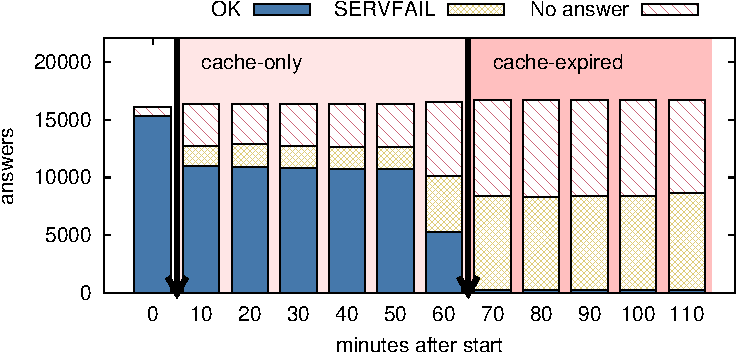
\includegraphics[width=0.7\columnwidth]{fig/hist.pdf}
 \caption{TTL: 1h; 100\%  Packet loss after $t=10$min}
\label{fig:class-valid-queries}
\end{figure}

\end{frame}


\begin{frame}
 \frametitle{R5: Consider longer TTL values whenever 
possible}
\begin{itemize}
 
 
 \item Caching is a \textit{key} component of resolver's resilience
   \item Retries as well -- to the point that resolvers may ``hammer'' 
authoritatives
   
   
 \item As such, \cite{Moura18b} recommend longer TTLs whenever possible
 
 
 \end{itemize}
 
 
\end{frame}

\begin{frame}
 \frametitle{R6:  Shared Infrastructure Risks Collateral Damage During 
Attacks}
 \begin{itemize}
  \item Be careful when contracting/engineering DNS services:
  
  \begin{itemize}
   \item  co-location implies you shared  (parts of the) infrastructure
  \end{itemize}


\item \cite{Moura16b} found that when Root DNS was attacked, some \url{.nl}
co-located sites were also down
\item Dyn 2016 Attack shows the same  
\begin{itemize}
 \item multiple zones partially reachable 
when NSes were attacked
\end{itemize}


\item OPS: be aware of shared infrastructure risk
 \end{itemize}

\end{frame}




\begin{frame}
 \frametitle{Questions?}

 \begin{itemize}
  \item R1: Use equaly strong IP anycast in every authoritative server to
    achieve even load distribution~\cite{Mueller17b}
    
  \item R2:  Routing Can Matter More Than Locations~\cite{Schmidt17a}
  
  \item R3: Collecting Detailed Anycast Catchment Maps Ahead of Actual
    Deployment Can Improve Engineering Designs~\cite{Vries17b}
    
  \item R4:    When under stress, employ two strategies~\cite{Moura16b}
  
  \item R5:  Consider longer time-to-live values whenever 
possible~\cite{Moura18b}
  
    \item R6:  Shared Infrastructure Risks Collateral Damage During 
Attacks~\cite{Moura16b}
    
 \vspace{1cm}
 \centering \textit{Thanks  reviewers of draft versions}
 \centering \small 
\url{https://github.com/gmmoura/draft-moura-dnsop-authoritative-recommendations}
  

 \end{itemize}

\end{frame}



% 
% \begin{frame}
%  \frametitle{Questions?}
%  
%  
%  \begin{itemize}
%   \item Draft on GitHub: \small
% \url{https://github.com/gmmoura/draft-moura-dnsop-authoritative-recommendations}
%  \end{itemize}
% 
% \end{frame}
 
 \begin{frame}[allowframebreaks] {References}
 
\bibliographystyle{IEEEtran}
% \balance
\small
\bibliography{subset,rfc}
\end{frame}
 
\end{document}
